\documentclass[slidestop,compress,mathserif]{beamer}
%\documentclass{beamer} 
\usepackage{beamerthemeshadow}
\usepackage[utf8]{inputenc}
\usepackage{listings}	%listingi
%\usepackage[T1]{polski}
%\usepackage[polski]{babel}	%znaki diaketryczne
\usepackage{polski}

%\usepackage[bars]{beamerthemetree} % Beamer theme v 2.2
\usetheme{Berlin}                  % Beamer theme v 3.0
%\usecolortheme{lily}                % Beamer color theme
\usepackage{color}

%\lstset{language=R,frame=ltrb,framesep=5pt,basicstyle=\normalsize,keywordstyle=\ttfamily\color{OliveGreen},identifierstyle=\ttfamily\color{CadetBlue}\bfseries,commentstyle=\color{Brown},stringstyle=\ttfamily,showstringspaces=ture}
\lstset{language=C++}

\title{TDD - Test Driven Development}
\author{Piotr Ślatała, Tomasz Żurkowski}
%\institute{}
\begin{document}
%\begin{frame}                       % Cover slide
\section{TDD}
%\subsection{Plan prezentacji}

\subsection{Wstęp}
\frame{
 \titlepage
}
%\end{frame}
% Instead, you can use \frame{\titlepage}} (Beamer v 2.2 macro)

\begin{frame}
 \frametitle{Plan prezentacji}
 \begin{enumerate}
 \item Idea testów
 \pause \item TDD
 \pause \item Frameworki do testowania
 \pause \item Mocki
 \pause \item Dependency Injection
\end{enumerate}

\end{frame}


%\begin{frame}
\begin{frame}
 \frametitle{Wstęp}
\begin{enumerate}
 \item Co rozumiemy pod pojęciem testu? % pytanie do publiczności...
 \pause \item Co i po co testujemy? % weryfikacja poprawności, sprawdzenie działania, rodzaje testów
\end{enumerate}
\end{frame}

\begin{frame}
\frametitle{Etapy tworzenia oprogramowania}
\begin{enumerate}
\pause \item Analiza
\pause \item Projektowanie
\pause \item Implementacja
\end{enumerate}
\end{frame}

\begin{frame}
\frametitle{Rodzaje testów}
 \begin{enumerate}
  \item Testy jednostkowe
  \pause \item Testy integracyjne
  \pause \item Testy akceptacyjne (funkcjonalne)
  % nie gwarantują poprawności
  % jeśli coś zepsujemy, to widzimy, o ile wszystkie testy są napisane!
\end{enumerate}
\end{frame}
\note{
Testy akcepacyjne - powstają na etapie analizy wymagań. Dzięki nim, wiemy czego użytkownik się spodziewa i czy spełniamy jego wymagania
Testy integracyjne - powstają na etapie projektowania.
Testy jednostkowe - kodowanie
}

%\defverbatim[colored]\proccode{%
%   \begin{lstlisting}[frame=single,emph={ga},emphstyle=\color{olive}]
%int dlugosc = dlugoscTekstu(string);
%string kawalek = kawalekTekstu(string, od, do);
%bool porownanie = porownajDwaTeksty(string1, string2);
%\end{lstlisting}}%
%\defverbatim[colored]\oopcode{%
% \begin{lstlisting}[frame=single,emph={ga},emphstyle=\color{olive}]
%int dlugosc = string.Dlugosc();
%string kawalek = string.Wytnij(od, do);
%bool porownanie = string1.JestRowny(string2);
%\end{lstlisting}}%
%\frame{%
%   \frametitle{Przykład proceduralny oraz OOP}
%   \proccode
%   \oopcode
%}%

\begin{frame}
\frametitle{Test driven development}
Proces normalny
 \begin{enumerate}
  \item Design aplikacji
  \pause \item Implementacja
  \pause \item Testy 
\end{enumerate}
\end{frame}

\begin{frame}
\frametitle{Test driven development}
Test driven development
 \begin{enumerate}
  \item Testy
  \pause \item Minimum kodu
  \pause \item Design %jako skutek uboczny ;)
\end{enumerate}
\end{frame}

\begin{frame}
\frametitle{Test driven development}
Czyli innymi słowy
 \begin{enumerate}
\item Implementujemy testy z wykorzystaniem nieistniejących obiektów.
\pause \item Generujemy niezbędne "stuby"
\pause \item Uruchamiamy testy
\end{enumerate}
\pause
\begin{block}{Krok 1}
	\textcolor{red}{RED}
\end{block}
\pause
\begin{block}{Krok 2}
	\textcolor{green}{GREEN}
\end{block}
\pause
\begin{block}{Krok 3}
 Refactor
\end{block}
\end{frame}

\begin{frame}
 \frametitle{TDD Cycle}
\begin{figure}
 \centering
 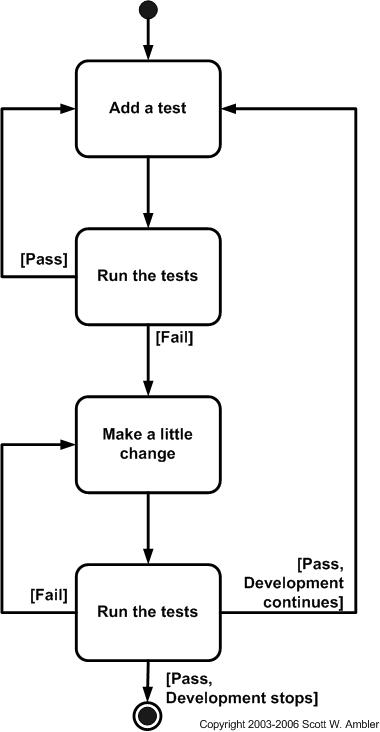
\includegraphics[height=190pt]{tddSteps.jpg}
\end{figure}
\end{frame}

\begin{frame}
 \frametitle{TDD Cycle}
\begin{figure}
 \centering
 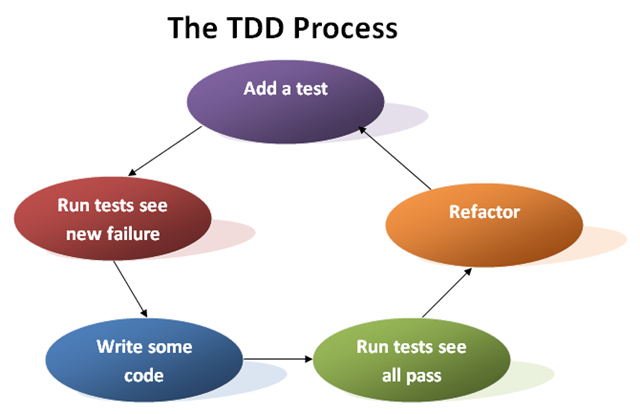
\includegraphics[width=250pt]{tddSteps.png}
\end{figure}
\end{frame}

\begin{frame}
 \frametitle{Korzyści wynikające z TDD}
 \begin{itemize}
 \item Dobry design ;-) %poprzez częste refactorowanie możemy zapewnić dobry design aplikacji, 
 \pause \item Szukanie błędów
 \pause \item Wysoka jakość kodu
 \pause \item ...
 \end{itemize}
\end{frame}

\section{Frameworki}
\subsection{Unit test frameworks}
\begin{frame}
	\frametitle{Frameworki ułatwiające testowanie}
	\begin{itemize}
		\item{MbUnit (Gallio)}
		\pause \item{NUnit}
		\pause \item{Visual Unit}
	\end{itemize}
\end{frame}

\subsection{Unit test frameworks overview}
\begin{frame}
	\frametitle{Frameworki ułatwiające testowanie}
	\begin{itemize}
		\item{Atrybuty}
			\begin{itemize}
				\pause \item{TestFixture}
				\pause \item{Test}
				\pause \item{SetUp}
				\pause \item{TearDown}
			\end{itemize}
		\pause \item{Asserty}
			\begin{itemize}
				\pause \item{AreEquals}
				\pause \item{AreAproximatelyEquals}
				\pause \item{Throws}
				\pause \item{i dużo więcej ...}
			\end{itemize}
	\end{itemize}
\end{frame}
	
\subsection{Mock frameworks}
\begin{frame}
	\frametitle{Frameworki do mocków}
	\begin{itemize}
		\item{Moq}
		\pause \item{NMock}
		\pause \item{EasyMock.Net}
		\pause \item{TypeMock Isolator (Commercial)}
		\pause \item{Rhino Mocks}
	\end{itemize}
\end{frame}

\subsection{Acceptance tests frameworks}
\begin{frame}
	\frametitle{Frameworki do testów akceptacyjnych}
	\begin{itemize}
		\item{Selenium}
		\pause \item{WatiN}
		\pause \item{White}
	\end{itemize}
\end{frame}

\section{Dependency Injection}
\subsection{Dependency Injection}
\begin{frame}
	\frametitle{Dependency Injection}
	\begin{itemize}
		\pause \item O co im znowu chodzi? %czyli wstrzykiwanie zależności
		\pause \item Kontenery %:]
		\pause \begin{itemize}
			\item Castle Windsor
			\item StructureMap
			\item Ninject, Spring.Net, PicoContainer.Net ....
		\end{itemize}
	\end{itemize}
\end{frame}
	
\section{Demo}
\subsection{Demo}
\begin{frame}
	\frametitle{Demo}
	\begin{center}
		\huge{Demo}
	\end{center}
\end{frame}
	
	
\end{document}
